%%%%%%%%%%%%%%%%%%%%%%%%%%%%%%%%%%%%%%%%%
% Beamer Presentation
% LaTeX Template
% Version 1.0 (10/11/12)
%
% This template has been downloaded from:
% http://www.LaTeXTemplates.com
%
% License:
% CC BY-NC-SA 3.0 (http://creativecommons.org/licenses/by-nc-sa/3.0/)
%
%%%%%%%%%%%%%%%%%%%%%%%%%%%%%%%%%%%%%%%%%

%----------------------------------------------------------------------------------------
%	PACKAGES AND THEMES
%----------------------------------------------------------------------------------------

\documentclass{beamer}

\mode<presentation> {

% The Beamer class comes with a number of default slide themes
% which change the colors and layouts of slides. Below this is a list
% of all the themes, uncomment each in turn to see what they look like.

%\usetheme{default}
%\usetheme{AnnArbor}
%\usetheme{Antibes}
%\usetheme{Bergen}
\usetheme{Berkeley}
%\usetheme{Berlin}
%\usetheme{Boadilla}
%\usetheme{CambridgeUS}
%\usetheme{Copenhagen}
%\usetheme{Darmstadt}
%\usetheme{Dresden}
%\usetheme{Frankfurt}
%\usetheme{Goettingen}
%\usetheme{Hannover}
%\usetheme{Ilmenau}
%\usetheme{JuanLesPins}
%\usetheme{Luebeck}
%\usetheme{Madrid}
%\usetheme{Malmoe}
%\usetheme{Marburg}
%\usetheme{Montpellier}
%\usetheme{PaloAlto}
%\usetheme{Pittsburgh}
%\usetheme{Rochester}
%\usetheme{Singapore}
%\usetheme{Szeged}
%\usetheme{Warsaw}

% As well as themes, the Beamer class has a number of color themes
% for any slide theme. Uncomment each of these in turn to see how it
% changes the colors of your current slide theme.

%\usecolortheme{albatross}
%\usecolortheme{beaver}
%\usecolortheme{beetle}
%\usecolortheme{crane}
\usecolortheme{dolphin}
%\usecolortheme{dove}
%\usecolortheme{fly}
%\usecolortheme{lily}
%\usecolortheme{orchid}
%\usecolortheme{rose}
%\usecolortheme{seagull}
%\usecolortheme{seahorse}
%\usecolortheme{whale}
%\usecolortheme{wolverine}

%\setbeamertemplate{footline} % To remove the footer line in all slides uncomment this line
%\setbeamertemplate{footline}[page number] % To replace the footer line in all slides with a simple slide count uncomment this line

%\setbeamertemplate{navigation symbols}{} % To remove the navigation symbols from the bottom of all slides uncomment this line
}

\usepackage{graphicx} % Allows including images
\usepackage{booktabs} % Allows the use of \toprule, \midrule and \bottomrule in tables
\usepackage[utf8]{inputenc}
\usepackage{multirow}

%----------------------------------------------------------------------------------------
%	TITLE PAGE
%----------------------------------------------------------------------------------------

\title[EP1]{EP2 - MAC0422} % The short title appears at the bottom of every slide, the full title is only on the title page

\author{João Gabriel e Juliano Garcia} % Your name
\institute[IME- USP] % Your institution as it will appear on the bottom of every slide, may be shorthand to save space
{
Instituto de Matemática e Estatística - USP \\ % Your institution for the title page
}
\date{} % Date, can be changed to a custom date

\begin{document}

\begin{frame}
\titlepage % Print the title page as the first slide
\end{frame}

\begin{frame}
\frametitle{Overview} % Table of contents slide, comment this block out to remove it
\tableofcontents % Throughout your presentation, if you choose to use \section{} and \subsection{} commands, these will automatically be printed on this slide as an overview of your presentation
\end{frame}

%----------------------------------------------------------------------------------------
%	PRESENTATION SLIDES
%----------------------------------------------------------------------------------------

%------------------------------------------------
\section{Estruturas}
%------------------------------------------------

\begin{frame}
\begin{center}
\huge Estruturas
\end{center}
\end{frame}

\begin{frame}
\frametitle{Estruturas de dados utilizadas}
\begin{itemize}
\item Buffer: É um buffer estático de pontuações, indicando a colocação dos ciclistas em determinada volta;
\item Pista (Road): É composta por uma matriz $dx10$ de identificadores inteiros, uma matriz $dx10$ de mutexes, e algumas variáveis de controle, como um vetor com a quantidade de ciclistas em cada faixa, variáveis que guardam as informações da entrada (número de ciclistas, tamanho da pista e número de voltas) e ponteiros para o grafo de dependência dos ciclistas e uma lista de pilhas;
\item Placar (Scoreboard): É composto por uma fila estática de buffers e mais algumas variáveis de controle, como o número de ciclistas ativos e o número de ciclistas que não quebraram;
\end{itemize}
\end{frame}

\begin{frame}
\frametitle{Estruturas de dados utilizadas}
\begin{itemize}
\item Digrafo (Graph): É um grafo de dependência utilizado para nos certificarmos de que os ciclistas não irão entrar em deadlock permanente;
\item Pilha (Stack): É uma pilha de inteiros utilizada em funções relacionadas ao grafo;
\item Lista de pilhas (Stacklist): Uma lista de pilhas utilizada para guardar os componentes fortemente conexos do grafo;
\item Ciclista (Biker): Uma estutura composta por um contador de voltas, a posição $(i, j)$ do ciclista, seu id, sua pontuação, sua velocidade, seu tempo, sua thread, 4 mutexes, e variáveis booleanas que indicam se ele já moveu e se seus mutexes já foram usados (explicado melhor nos próximos slides). 
\end{itemize}
\end{frame}

\begin{frame}
\frametitle{Decisões de implementação de fluxo}
\begin{itemize}
\item Além das threads dos ciclistas, utilizamos a thread da main para coordenar algumas operações durante a corrida, como debug e previsão de dependências ciclicas;
\item Utilizamos 3 barreiras de sincronização para sincronizar todas as n+1 threads (ciclistas + main): Uma para sincronizar os movimentos dos cicistas, outra para que as threads se preparem para a próxima iteração e para imprimir o debug e a terceira para que as threads acabem ao mesmo tempo no final do programa;
\item Utilizamos as barreiras disponíveis na biblioteca pthread. 
\end{itemize}
\end{frame}

%-------------------------------------------------
\section{Ciclistas}
%-------------------------------------------------

\begin{frame}
\begin{center}
\huge Ciclistas
\end{center}
\end{frame}

\begin{frame}
\frametitle{Decisões de implementação dos ciclistas}
\begin{itemize}
\item Ciclistas só se movimentam para posições adjacentes à eles na matriz (incluindo diagonais).
\item Ciclistas esperam os da frente para se movimentar.
\item Sempre que possível, respeitando as outras regras, os ciclistas vão em direção à pista mais interna.
\item Quando um ciclista quebra, criamos uma thread dummy que fica ativando as barreiras para que as outras threads continuem rodando.
\end{itemize}
\end{frame}

\begin{frame}
\frametitle{Loop dos ciclistas}
\begin{columns}[c]
\column{.3\textwidth}
\begin{figure}
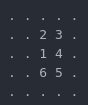
\includegraphics[scale=0.6]{biker_example.png}
\end{figure}
\column{.7\textwidth}
Na figura as posições que não são importantes estão representadas por "." e os ciclistas por números. O ciclista em foco é o número 1. As linhas representam as faixas e as colunas representam os metros. A faixa superior é a mais interna e os ciclistas se movem da esquerda para a direita.
\end{columns}
\vfill
Loop:
\begin{enumerate}
\item Espera os ciclistas que estão nas posições 2 (cima), 3 (diagonal superior direita), 4 (direita) e 5 (diagonal inferior direita) moverem para continuar.
\item Tenta se mover para a posição 3, se não conseguir tenta a 4 e se não conseguir tenta a 5.
\item Espera a barreira, e então volta para a instrução 1.
\end{enumerate}
\end{frame}

\begin{frame}
\frametitle{Grafo de dependência}
A relação de espera para executar o movimento pode ser representada em um grafo de dependência:
\begin{figure}
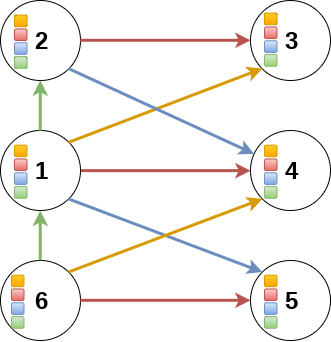
\includegraphics[scale=0.4]{dependency.png}
\end{figure}
\end{frame}


\begin{frame}
\frametitle{Regras extras}
Para evitar alguns comportamentos indesejados, adicionamos algumas regras extras:
\begin{itemize}
\item Um ciclista não pode mover para a posição 3 se houver um ciclista na posição 4, evitando ultrapassagens pela pista mais interna.
\item Um ciclista só pode mover para a posição 5 se o ciclista da posição 6 já se moveu, evitando que o ciclista bloqueie o ciclista da 6.
\item Um ciclista não pode mudar para uma faixa que tem d-1 ciclistas, nem esperar algum ciclista que está nela, evitando que não haja espaço para movimentação.
\item Se o ciclista pertence à um componente fortemente conexo (CFC) do grafo de dependência, com mais ou igual a $d$ vértices, ele não pode mudar nem esperar faixas que possuem ciclistas de algum CFC, evitando ciclos de dependência.
\end{itemize}
\end{frame}

\begin{frame}
\frametitle{Grafo de dependência e componente fortemente conexo}
Sem a última regra do slide anterior, seria possível que que os ciclistas entrassem em deadlock em ciclo esperando os da frente se moverem, como é mostrado nas imagens abaixo numa pista de tamanho 8.
\begin{columns}[c]
\column{.35\textwidth}
\begin{figure}
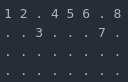
\includegraphics[scale=0.6]{loop_example.png}
\end{figure}
\column{.65\textwidth}
\begin{figure}
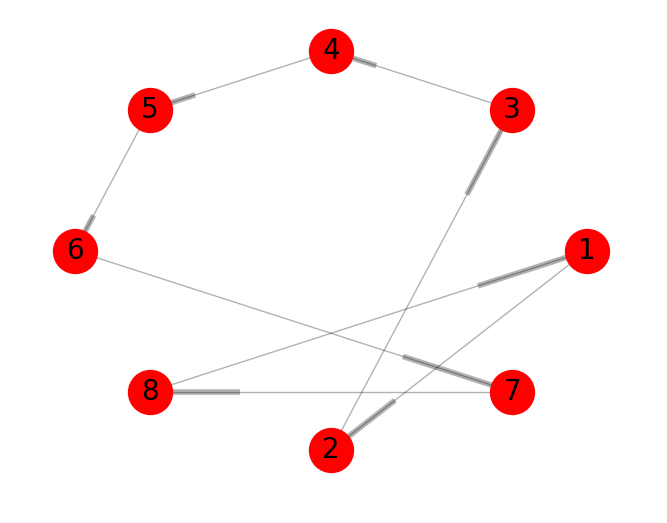
\includegraphics[scale=0.25]{depend_graph.png}
\end{figure}
\end{columns}
\end{frame}

\begin{frame}
\frametitle{Grafo de dependência e componente fortemente conexo}
Para isso, quando a pista tem mais de $d$ ciclistas, o programa traduz a pista para um digrafo de dependências e acha os componentes fortemente conexos dele utilizando o \textbf{Algoritmo de Tarjan} ($\mathcal{O}(n)$).
\\~\\
Nosso simulador identifica todos os ciclistas que pertencem a algum CFC que tenha quantidade de nós maior ou igual ao tamanho da pista ($d$) e aplica a regra do slide anterior, evitando que aconteça um ciclo de deadlock.
\end{frame}



%------------------------------------------------
\section{Gráficos}
%------------------------------------------------

\begin{frame}
\begin{center}
\huge Gráficos
\end{center}
\end{frame}

\begin{frame}
\frametitle{Gráficos}
Tamanho da pista (fixo) = 300
\\~\\
Quantidade de voltas:
\begin{itemize}
\item 20 (baixa)
\item 60 (média)
\item 80 (alta)
\end{itemize}
Quantidade de ciclistas:
\begin{itemize}
\item 40 (poucos)
\item 150 (médio)
\item 337 (muitos)
\end{itemize}
\end{frame}

\begin{frame}
\frametitle{Gráficos}
\begin{itemize}
\item O tempo foi medido usando o GNU time 1.7, com a opção 'e':
"Elapsed real (wall clock) time used by the process, in seconds"; 
\item A medição de memória foi feita utilizando o script bash \textbf{memusage}, e os dados apresentados são da seção 'heap total';
\item Nos gráficos a seguir, as linhas em preto representam o intervalo de confiança, e cada barra a média de 30 medições da respectiva categoria.
\end{itemize}
\end{frame}


\begin{frame}
\frametitle{Uso de tempo}
\begin{figure}
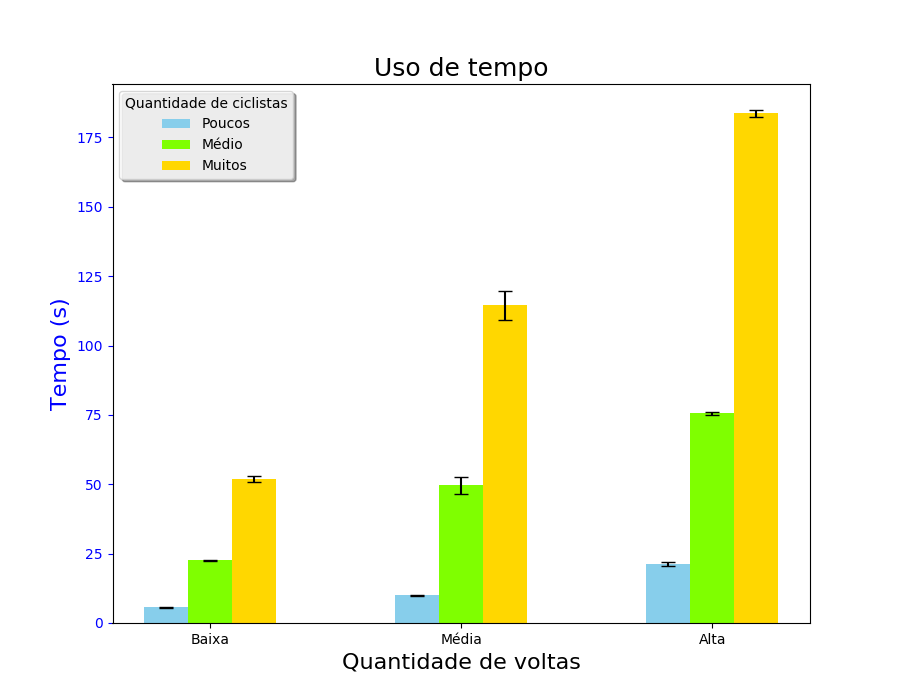
\includegraphics[scale=0.4]{time_usage.png}
\end{figure}
\end{frame}

\begin{frame}
\frametitle{Uso de memória}
\begin{figure}
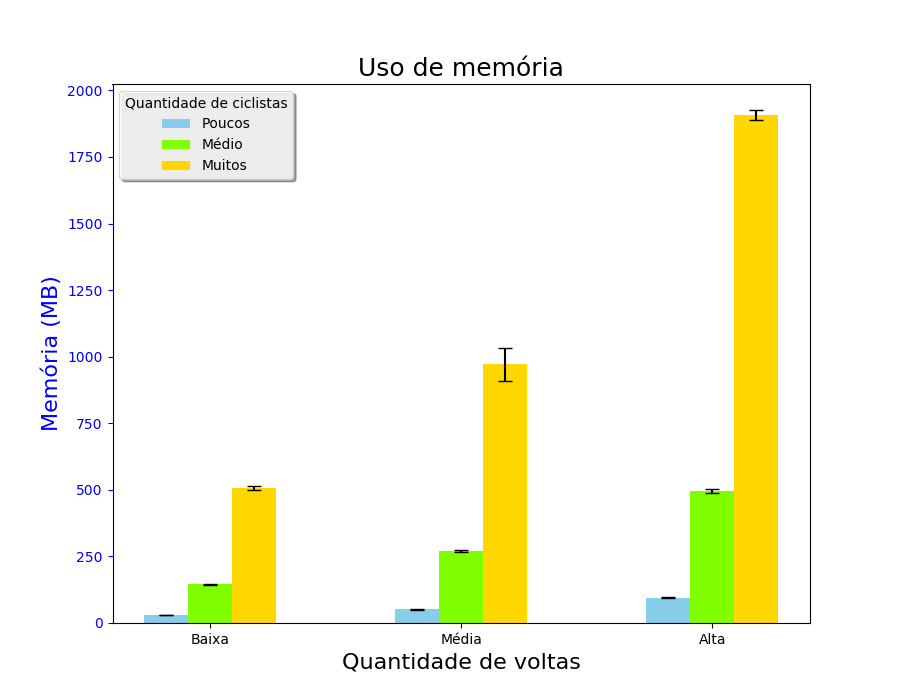
\includegraphics[scale=0.4]{mem_usage.png}
\end{figure}
\end{frame}

\begin{frame}
\frametitle{Conclusões}
Os resultados foram os esperados:
\begin{itemize}
\item Quanto maior a quantidade de voltas, maior a quantidade de tempo e maior a memória gasta (mais alocações / desalocações de memória para os buffers do placar);
\item Quanto maior a quantidade de ciclistas, maior o tempo de execução (mais threads para executar) e maior a memória gasta (para os buffers do placar e para o grafo de dependência).
\end{itemize}

\end{frame}

% Blocks:
%\begin{block}{Block 1}
%Lorem ipsum dolor sit amet, consectetur adipiscing elit. Integer lectus nisl, ultricies in feugiat rutrum, porttitor sit amet augue. Aliquam ut tortor mauris. Sed volutpat ante purus, quis accumsan dolor.
%\end{block}

% Paragraph division: \\~\\

% Columns
%\begin{columns}[c] % The "c" option specifies centered vertical alignment while the "t" option is used for top vertical alignment

%\column{.45\textwidth} % Left column and width
%\textbf{Heading}
%\begin{enumerate}
%\item Statement
%\item Explanation
%\item Example
%\end{enumerate}

%\column{.5\textwidth} % Right column and width
%Lorem ipsum dolor sit amet, consectetur adipiscing elit. Integer lectus nisl, ultricies in feugiat rutrum, porttitor sit amet augue. Aliquam ut tortor mauris. Sed volutpat ante purus, quis accumsan dolor.

%\end{columns}

\begin{frame}
\frametitle{Bibliografia}
\footnotesize {
\begin{thebibliography}{99} % Beamer does not support BibTeX so references must be inserted manually as below
\bibitem[Sedgewick, Robert and Wayne, Kevin]{p1} Sedgewick, Robert and Wayne, Kevin
\newblock Algorithms, 4th Edition.
\bibitem[Tanenbaum, Andrew S.]{p1} Tanenbaum, Andrew S.
\newblock Modern Operating Systems, 4th Edition.
\end{thebibliography}
}
\end{frame}

\end{document}